% !TeX spellcheck = en_US
\chapter{Mathematical Programing}
\label{ch:mathprog}

This chapter will deal with the simplest class of decision problems We assume:
\begin{itemize}
	\item A preference relation $\Pi$ with a known consistent utility function $u(f)$
	$$ \exists u: F \rightarrow \R : \Pi = \left\{(f,f') \in F \times F \mid u(f) \geq u(f')\right\} $$
	
	\item A certain environment: $|\Omega| = 1 \implies f(x, \bar \omega)$ reduces to $f(x)$; a single scenario, the impact $f$ depends only on the alternative $x$
	
	\item A single decision-maker: $|D| = 1 \implies \Pi_d$ reduces to $\Pi$
\end{itemize}

This class of problems reduces the decision problem to classical optimization: 
$$ \max_{x \in X} u(f) $$
We'll discuss a solving technique that is very general but complex and inefficient.

This class of problems is mainly treated in mathematical literature, where preference is expressed as a cost function, so the most common form is
$$ \min_{x \in X} f(x) $$
where $f(x)$  replaces $-u(f(x))$ (not the original $f$).

We also assume regularity for the objective and feasible region:
\begin{itemize}
	\item $f(x) \in C^1 (X)$; the cost function is continuous with its first derivative
	
	\item $X = \left\{x \in \R^n \mid g_j (x) \leq 0, \ j = 1, \dots, m\right\}$ with $g_j (x) \in C^1 (X)$; the solution set $X$ can be described through a finite system of inequalities, where the constraint functions $g_j(x)$ are real-valued continuous functions with a continuous first derivative in the feasible solution set of the problem
\end{itemize}

These are very general assumptions. This class of problem (with assumptions more or less strict with respect to the continuity of functions) are denoted under the label of \textbf{Mathematical Programming} problems, describing both preference and feasible region through real-valued functions allows to apply mathematical analysis to these decision problems.

\section{Basic concepts}
\label{sec:mathbasic}

\begin{definition}
	Given a set $X \subseteq \R^n$ and a function $f: X \rightarrow \R$ we denote as \textbf{global optimum point} a point $x^\circ \in X$ such that
	$$ f\left(x^\circ \right) \leq f(x) \quad \forall x \in X $$
\end{definition}

\begin{definition}
	Given a set $X \subseteq \R^n$ and a function $f: X \rightarrow \R$, we denote as \textbf{local optimum point} a point $x^\ast \in X$ such that 
	$$ \exists \epsilon > 0 : f\left(x^\ast\right) \leq f(x), \quad \forall x \in X \cap \U_{x^\ast, \epsilon} $$
	where
	$$ \U_{x^\ast, \epsilon} = \left\{x \in \R^n \mid \| x - x^\ast \| < \epsilon \right\} $$
	is a neighborhood of $x^\ast$ of width $\epsilon$ ($\|x - x^\ast \|$ is the norm of vector $x - x^\ast$).
\end{definition}

It can easily be seen that a global optimum is, by definition, also a local optimum:
$$ X^\circ \subseteq X^\ast $$

There is no process to find $X^\circ$ or $X^\ast$ directly, so we want to search the conditions necessary for local optimality. These conditions aim to identify points "candidate" to being local optimum, weakening twice our request:
$$ 
\begin{array}{c c c c c}
	\text{Global optimum} & \implies & \text{Local optimum} & \implies & \text{KKT conditions} \\
	$X^\circ$ & \subseteq & X^\ast & \subseteq & X^{KKT} 
\end{array}
$$
The conditions are known as \textbf{Karush-Kuhn-Tucker conditions}, from the names of their discoverers.

After finding the "weakened" set, we enumerate $X^{KKT}$ exhaustively to find $X^\circ$. 

The KKT conditions identify candidate points as follows: 
\begin{enumerate}
	\item Lay out the conditions as a system of equalities and inequalities
	
	\item Solve the system, finding $X^{KKT}$
	
	\item Evaluate every point in $X^{KKT}$, keeping only the best ones (which will compose $X^\circ$)
\end{enumerate}

The method requires $X^{KKT}$ to be a finite set, or at least a set which can be analytically describes, in order to determine $X^\circ$.

The basic tool will be linear approximation in small neighborhoods (hence the false positives).

\subsection{Taylor's series expansion}
\label{subsec:taylor}

Every sufficiently regular function (i.e., continuous function with continuous derivatives up to a suitable order $k$) can be locally approximated with a polynomial of degree $k$. \\

\begin{theo}
	Let $f \in C^k \left(\U_{\tilde x, \epsilon}\right)$ be a function of a real variable $x \in \R$. For all $x \in \U_{\tilde x, \epsilon}$, Taylor's series expansion holds: 
	$$ f(x) = \sum_{i = 0}^k \frac{f^{(i)} (\tilde x)}{i!} (x - \tilde x)^i $$ 
	$$ \text{with } f^{(0)}  = f, \quad f^{(i)} = \frac{d^i f}{dx^i} \quad \forall i \in \N^+, \text{ and } \lim_{x \rightarrow \tilde x} \frac{R_k (x - \tilde x)}{\|x - \tilde x\|} = 0$$
\end{theo}

Any regular function can be locally approximated in $\tilde x$ by its tangent line, terms with exponents higher than 1 improve the approximation (which we'll not consider). Any function regular up to the first order ($f: \R \rightarrow \R$ and $f \in C^1 (\U_{\tilde x, \epsilon})$) admits a linear approximation
$$ f(x) = f(\tilde x) +  f'(\tilde x) (x - \tilde x)  + R_1 (|x - \tilde x|)$$
which can be generalized to multiple-variable functions ($x \in \R^n$) by 
$$ f(x) = f(\tilde x) + \left(\nabla f(\tilde x)\right)^T (x  - \tilde x) + R_1 (\|x - \tilde x\|) $$
where 
$$ \lim_{x \rightarrow \tilde x} \frac{R_1 \left(\|x - \tilde x\|\right)}{\|x - \tilde x\|} = 0$$
and $\nabla f(x)$ is the gradient vector
$$ 
\nabla f(x) = \left[\begin{array}{c}
	\frac{\partial f}{\partial x_1} \\ \dots \\ \frac{\partial f}{\partial x_n}
\end{array}\right]
$$
It's the direction of quickest increase for $f(\cdot)$.

\subsection{Arcs}
\label{subsec:arcs}

$\R^n$ offers many ways to move away from $\tilde x$.\\

\begin{definition}
	Given a point $\tilde x \in \R^n$, an \textbf{arc} in $\tilde x$ is a parametric curve $\xi: \R^+ \rightarrow \R^n$, that is $\xi (\alpha) = \left[\begin{array}{c}
		\xi_1 (\alpha) \\ \dots \\ \xi_n (\alpha)
	\end{array}\right]$, such that $\xi (0) = \tilde x$ and $\xi_1 (\alpha) \in C^1 (\R^+)$.
\end{definition}

Basically, a function that starts at $\tilde x$ (since $\xi (0) = \tilde x$) and then gets further from it, with each component continuously differentiable for $\alpha > 0$. \\

\begin{definition}
	An arc $\xi (\alpha)$ is \textbf{feasible} for a given region $X \subseteq \R^n$ when the curve remains in $X$ for small $\alpha$
	$$ \exists \bar \alpha_f > 0 : \xi (\alpha) \in X, \quad \forall \alpha \in [0; \bar \alpha_f) $$
\end{definition}

Given a region $X$ (our function), we can travel "a little" (a small enough interval, as defined) along the arc without leaving $X$. \\

\begin{definition}
	An arc $\xi (\alpha)$ is \textbf{improving} for a given function $f:X \rightarrow \R$ when $f$ is strictly better in $\xi (\alpha)$ than in $\tilde x$ for all small positive $\alpha$
	$$ \exists \bar \alpha_i > 0 : f\left(\xi(\alpha)\right) < f (\tilde x), \quad \forall \alpha \in (0; \bar \alpha_i) $$
\end{definition}

Along the curve, but close enough to $\tilde x$, the value of the function $f$ is strictly better than in $\tilde x$.

\section{Necessary conditions for local optimality}
\label{sec:necforlocal}

\begin{theo}
	If $\tilde x \in X \subseteq \R^n$ (a point in a region), $f(\cdot) \in C^1 (X)$ (continuously differentiable function) and $\xi (\alpha)$ is an arc in $\tilde x$, feasible for $X$ and improving for $f(\cdot)$, then $\tilde x$ is not locally optimal for $f(\cdot)$ in $X$.
\end{theo}

If a feasible improving arc in $\tilde x$ exists, then $\tilde x$ can't be a local optima; no improving arc can exist ar a local optima.

\begin{proof}
	By assumption, for suitable values $\bar \alpha_f > 0$ and $\bar \alpha_i > 0$, we have:
	\begin{itemize}
		\item $\xi (\alpha)$ feasible: $\xi (\alpha) \in X$ for all $\alpha \in [0, \bar \alpha_f)$
		
		\item $\xi (\alpha)$ improving: $f(\xi(\alpha))  < f(\tilde x)$ for all $\alpha \in (0, \bar \alpha_i)$
	\end{itemize}
	
	Since $\xi (\alpha)$ is a continuous arc 
	$$ \lim_{\alpha \rightarrow 0} \xi(\alpha) = \tilde x \Leftrightarrow \forall \epsilon > 0, \ \exists \bar \alpha_\epsilon  : \| \xi(\alpha)  - \tilde x \| < \epsilon, \ \forall \alpha \in (0, \bar \alpha_\epsilon ) $$
	that is, $\xi (\alpha) \in \U_{\tilde x, \epsilon}$, $\forall \alpha \in (0, \bar \alpha_\epsilon )$.
	
	Now $\alpha = \frac{1}{2} \min (\bar \alpha_f, \bar \alpha_i \bar \alpha_\epsilon )$ satisfies all three conditions: 
	\begin{itemize}
		\item $\alpha < \bar \alpha_f \implies \xi(\alpha) \in X$
		
		\item $\alpha < \bar \alpha_i \implies f(\xi(\alpha)) < f(\tilde x)$
		
		\item $\alpha < \bar \alpha_\epsilon \implies \xi(\alpha) \in \U_{x^\ast, \epsilon}$
	\end{itemize}
	But this contradicts local optimality
	$$ f(x) \geq f(\tilde x), \quad \forall x \in \U_{\tilde x, \epsilon}  \cap X $$
\end{proof}

\subsection{A filtering approach}
\label{subsec:filteringapproach}

This suggests an approach to find candidate points: remove from $X$ all the points that are provably nonoptimal:
\begin{enumerate}
	\item Consider all feasible points as candidates: $C := X$
	
	\item Scan the set of candidate points $C$
	
	\item For each candidate point $\tilde x$, scan all feasible arcs
	
	\item For each arc $d$ feasible in $\tilde x$, check whether the arc is improving for $f(\cdot)$: if it is, remove $\tilde x$ from the candidate set
	
	\item In the end, scan the remaining candidate points, keeping only the best ones
\end{enumerate}

The pseudo-code of which being:
\begin{myalgo}{0.85}
	$X^{KKT} := X$; \\
	\tcp{(continuous set for $x$)}
	\For{\texttt{each} $x \in X^{KKT}$}{
		\tcp{(continuous set for $\xi$, interval for $\alpha$)}
		\For{\texttt{each} arc $\xi(\alpha)$ in $x$ feasible for $X$}{
			\tcp{(interval for $\alpha$)}
			\If{$\xi(\alpha)$ is improving in $x$ for $f(\cdot)$}{
				$X^{KKT}:=X^{KKT} \setminus \{x\}$; \\
			}
		}
	}
	\Return{$X^{KKT}$;}
\end{myalgo}

Problem: the set of feasible points and directions is, generally, infinite. We can replace the infinite loops with more efficient analytic conditions, all based on first-order approximations. \\

\begin{definition}
	We denote as \textbf{tangent direction} of an arc $\xi (\alpha)$ feasible in $\tilde x$ the vector composed of the first derivatives of the components $\xi_i$ with respect to parameter $\alpha$, evaluated in the starting point of the arc
	$$ p_\xi = \left[\begin{array}{c}
		\xi_1'(0) \\ \dots \\ \xi_n'(0) \\
	\end{array}\right]$$
\end{definition}

Straight lines $\xi (\alpha) = \tilde x + \alpha d$ have tangent direction $d$ (\textit{arcs generalize directions}).

Example: the arc in $\tilde x = (2,0)$
$$ \xi (\alpha) = \left[\begin{array}{c}
	2 \cos \alpha \\ 2 \sin \alpha 
\end{array}\right] $$
describes the circumference with center in the origin and radius 2. Its tangent direction is 
$$ p_\xi = \left[\begin{array}{c}
	-2 \sin 0 \\ 2 \cos 0
\end{array} \right] = \left[ \begin{array}{c}
0 \\ 2
\end{array}\right] $$

\begin{theo}
	If $x^\ast$ is locally optimal in $X$ for $f(\cdot)$ and $\xi (\alpha)$ is a feasible arc in $x^\ast$ for $X$, then 
	$$ \nabla f (\tilde x)^T p_\xi \geq 0 $$
\end{theo}

\begin{proof}
	If $\xi (\alpha)$ is a feasible arc, there exists a coefficient $\bar \alpha$ such that $\xi (\alpha) \in X$ for all $\alpha \in [0;\bar \alpha)$ (remains in $X$ for a small $\alpha$) and since $x^\ast$ is a local optima, for small $\alpha$ it holds that $f(\xi (\alpha)) \geq f(x^\ast)$. 
	
	Apply Taylor's expansion to $f(\xi (\alpha))$ in $\alpha = 0$
	\begin{align*}
		f(\xi (\alpha)) & \geq f(x^\ast) \implies \\
		\implies \cancel{f(\xi (0))} + \left \frac{df}{d\alpha} \right|_{\alpha = 0} \alpha + R_1 \left(\|\xi(\alpha) - \xi (0) \|\right) & \geq \cancel{f(x^\ast)} \implies  \\
		\implies \left(\nabla f(x^\ast)\right)^T  p_\xi + \frac{R_1 \left(\| \xi (\alpha)  - \xi (0) \| \right)}{\alpha} & \geq 0 \\
	\end{align*}
	
	If $\alpha$ converges to 0, by continuity the inequality is preserved
	$$ \lim_{\alpha \rightarrow 0} \left( \left(\nabla f(\tilde x)\right)^T p_\xi + \frac{R_1 \left( \xi (\alpha) - \xi (0)\right)}{\| \xi (\alpha) - \xi (0) \|} \frac{\| \xi (\alpha) - \xi (0) \|}{\alpha}\right) \geq 0 \implies $$
	$$ \implies \left(\nabla f(\tilde x)\right)^T p_\xi \geq 0 $$
\end{proof}

Example: 
\begin{align*}
	\min f(x) & = x_2 \\ g_1 (x) & = x_1^2 + x_2^2 \ \leq 4
\end{align*}
with $\nabla f^T = [0 \ 1]$
\begin{itemize}
	\item Arc $\xi (\alpha) = \tilde x + \alpha [1 \ -1]^T$ is improving in $\tilde x = (-2, 0)$: therefore $\tilde x$ is not locally optimal
	$$ \nabla f (-2, 0)^T p_\xi = [0 \ 1] \cdot [1 \ -1]^T = -1 < 0 $$
	
	\item Arc $\xi (\alpha) = \tilde x + \alpha[1 \ 1]^T$ is nonimproving in $\tilde x = (0, -2)$: $\tilde x$ could be locally optimal (remains candidate until disproval)
	$$ \nabla f(0, -2)^T p_\xi = [0 \ 1] \cdot [1 \ 1]^T = 1 \geq 0 $$ 
\end{itemize}

%I don't get the "intuitive" reason this is true, to me it's just a formula

The earlier code can be simplified (possibly missing some removals) to
\begin{myalgo}{0.85}
	$X^{KKT} := X$; \\
	\tcp{(continuous set for $x$)}
	\For{\texttt{each} $x \in X^{KKT}$}{
		\tcp{(continuous set for $\xi$, interval for $\alpha$)}
		\For{\texttt{each} arc $\xi(\alpha)$ in $x$ feasible for $X$}{
			\tcp{($\xi (\alpha)$ is improving in $x$ for $f(\cdot)$)}
			\If{{\color{red} $\nabla f(\tilde x)^T p_\xi < 0$}}{
				$X^{KKT}:=X^{KKT} \setminus \{x\}$; \\
			}
		}
	}
	\Return{$X^{KKT}$;}
\end{myalgo}

\subsection{Feasibility condition}
\label{subsec:feasibilitycondition}

Given the analytic description of the feasible region
$$ X = \left\{x \in \R^n \mid g_j (x) \leq 0 \text{ for } j = 1, \dots, m \right\}$$
we approximate each function $g_j(\cdot)$ with Taylor's expansion.

However, feasibility differs from improvement in two regards: 
\begin{itemize}
	\item It involves many inequalities, instead of a single objective
	
	\item It requires weak conditions, instead of a strict one \\
\end{itemize}

\begin{definition}
	We denote as \textbf{active constraint} in a point $\tilde x \in X$ any constraint $g_j (x) \leq 0$ such that $g_j (\tilde x) = 0$. We'll indicate by $J_a (x) = \left\{j \in \{1, \dots, m\}: g_j (x) = 0\right\}$ the set of indices of the active constraints.
\end{definition}

Basically, the constraints exactly equal to zero when considered in point $\tilde x$, and $J_a$ is the set of indices for which this condition holds.

Given point $\tilde x$ we partition the constraints into two classes
\begin{enumerate}
	\item The \textbf{active constraints} ($J_a (\tilde x)$) are exactly satisfied: $g_j (\tilde x) = 0$
	
	\item The nonactive constraints are largely satisfied: $g_j (\tilde x) < 0$
\end{enumerate}

Example: 
\begin{align*}
	\min f(x) & = (x_1 - 1)^2 + x_2 \\
	g_1 (x) & = -x_1^2 - x_2^2 + 4 \leq 0 \\
	g_2 (x) & = x_1 - 3/2 \leq 0
\end{align*}

Active constraints: 
\begin{itemize}
	\item for $x = (-2,-2)$, no active constraints: $J_a (-2, -2) = \emptyset$
	
	\item for $x = (3/2, 0)$, one active constraint: $J_a (3/2, 0) = \{2\}$
	
	\item for $x = (3/2, \sqrt{7}/2)$, two active constraints: $J_a (3/2, \sqrt{7}/2) = \{1,2\}$ \\
\end{itemize}

\begin{theo}
	If $\xi (\alpha)$ is a feasible arc in $\tilde x \in$ for $X$, $p_\xi$ its tangent vector. Then
	$$ \nabla g_j (\tilde x)^T p_\xi \leq 0, \quad \forall j \in J_a (\tilde x) $$
\end{theo}
\begin{proof}
	If $\xi (\alpha)$ is an arc feasible in $\tilde x$, there exists a coefficient $\bar \alpha$ such that
	$$ g_j (\xi (\alpha)) \leq 0, \quad \forall \alpha \in [0; \bar \alpha) \text{ and } j = 1, \dots, m $$
	that is
	\begin{align*}
		g_j (\xi (\alpha)) & = g_j (\xi(0)) + \left \frac{dg_j}{d \alpha}\right|_{0} \alpha + R_1 (\|\xi(\alpha) - \xi(0) \|) = \\
		& = g_j (\tilde x) + \alpha (\nabla g_j(\tilde x))^T p_\xi + R_1 (\| \xi(\alpha) - \xi (0)\|) \leq 0
	\end{align*}
	
	The inequality is obvious for all constraints not active in $\tilde x$ and the other two terms converge to zero as $\alpha \rightarrow 0$. Therefore, by continuity, when $\alpha$ is sufficiently small, they cannot reverse the inequality. 
	
	For the constraints which are active in $\tilde x$, on the contrary, the inequality introduces a strict condition, in fact, for such constraints $g_j(\tilde x) = 0$ so that
	$$ g_j (\xi (\alpha)) = \alpha (\nabla g_j (\tilde x))^T p_\xi + R_1 (\|\xi (\alpha) - \xi (0) \|) \leq 0 $$
	Dividing both terms by $\alpha$ and considering the limit, by continuity the thesis follows
	$$ \lim_{\alpha \rightarrow 0} \left[(\nabla g_j (\tilde x))^T p_\xi + \frac{R_1 (\| \xi (\alpha) - \xi (0) \|)}{\| \xi(\alpha) - \xi (0) \|} \frac{\| \xi (\alpha) - \xi (0) \|}{\alpha} \right] = (\Delta g_j (\tilde x))^T p_\xi \leq 0$$
\end{proof}

For any feasible arc $\xi (\alpha)$, vector $p_\xi$ satisfies the conditions above, but a vector $p$ that satisfies them is not always tangent to a feasible arc. Luckily, the problem concerns only some degenerate points.

\subsubsection{Regular points}

\begin{definition}
	We denote as \textbf{regular point} for a given system of constraints $g_j (x) \leq 0$a point in which all active constraint have linearly independent gradients (\textbf{constraint qualification} condition).
\end{definition}

In a regular point, the conditions on the gradients of the active constraints are not only necessary, but also sufficient to guarantee that there exists a feasible arc with the given tangent vector. \\

\begin{theo}
	If $\tilde x$ is a regular point, then $\nabla g_j (\tilde x)^T p \leq 0$ for all $j \in J_a (\tilde x)$ if and only if there exists an arc $\xi (\alpha)$ in $\tilde x$ feasible for $X$ with tangent direction $p_\xi = p$.
\end{theo}

The necessary conditions for feasibility are also sufficient in regular points. The analytical conditions on the gradients can be used to check feasibility in all regular points, nonregular points must be explicitly tested (candidates by default). \\

\begin{coro}
	\label{cor:firstgeo}
	Let $f \in C^1 (X)$, $\tilde x \in X$ be a regular and local optimum point and $p$ a vector such that
	$$ (\nabla g_j (\tilde x))^T p \leq 0, \quad \forall j \in J_a (\tilde x) $$
	Then 
	$$ (\nabla f(\tilde x))^T p \geq 0 $$
\end{coro}

The code now becomes:
\begin{myalgo}{0.85}
	$X^{KKT} := X \setminus$ NonRegular$(g, X)$; \\
	\tcp{(continuous set for $x$)}
	\For{\texttt{each} $x \in X^{KKT}$}{
		\tcp{(arc $\xi (\alpha)$ in $x$ feasible for $X$)}
		\For{\texttt{each} {\color{red} $p \in \R^n : \nabla g_j (x)^T p \leq 0$, $\forall j \in J_a (x)$}}{
			\tcp{($\xi (\alpha)$ is improving in $x$ for $f(\cdot)$)}
			\If{{\color{red} $\nabla f(\tilde x)^T p_\xi < 0$}}{
				$X^{KKT}:=X^{KKT} \setminus \{x\}$; \\
			}
		}
	}
	$X^{KKT} := X^{KKT} \cup $ NonRegular$(g,X)$; \\
	\Return{$X^{KKT}$;}
\end{myalgo}

\subsubsection{Special case: equality constraints}
\label{subsub:equalityconstraintsreplaced}
Special case: equality constraints $h_i (x) = 0$ are always active and can be treated as pairs of active inequalities: $h_i (x) \leq 0$ and $-h_i (x) \leq 0$
$$
\begin{cases}
	\nabla h_i (\tilde x)^T p_\xi & \leq 0 \\
	- \nabla h_i (\tilde x)^T p_\xi & \leq 0 \\
\end{cases}
\implies \nabla h_i (\tilde x)^T p_\xi = 0
$$

%Should be end of L7, notes p128

\subsection{A first geometric interpretation}
\label{subsec:firstgeometricinterpretation}

The property of Corollary \ref{cor:firstgeo} has a geometric interpretation that makes it quite intuitive. For each point $x$ taken into account, two sets of vectors are considered: 
\begin{enumerate}
	\item The \textbf{feasible cone} $C_{feas} (x)$ is the set of vectors that form angles $\geq 90^\circ$ with the gradients of all active constraints
	$$ (\nabla g_j (x))^T p \leq 0, \quad \forall j \in J_a (x) $$
	It's a cone because each active constraint identifies a half-space of directions pointing "on the opposite side" of its gradient, and intersecting them yields a cone. In regular points, these are the directions tangent to feasible arcs.
	
	\item The \textbf{improving half-space} $C_{impr} (x)$: it's the set of vectors that form angles $> 90^\circ$ with the gradient of the objective function
	$$ (\nabla f(x))^T p < 0 $$
\end{enumerate}

Corollary \ref{cor:firstgeo} states \textit{the feasible cone must not intersect the improving half-space}. Notice that the former is closed, whereas the latter is open, so that the two sets can touch, but not share internal points. The reason is that the directions in which the two cones touch have zero scalar product with the gradient of the objective and with the gradient of the active constraints; in that case, the first order information is insufficient to determine whether the direction is actually improving or not and actually feasible or not. Therefore, such points cannot be rejected and must remain candidate.

\section{Karush-Kuhn-Tucker conditions}
\label{sec:kktcond}

We want to turn the conditions of Corollary \ref{cor:firstgeo} into computationally tractable equivalent conditions, that is into solution of a system of equalities and inequalities. 

We have modified the filtering approach using analytic conditions: 
\begin{itemize}
	\item nonregular points are identified and considered as candidates
	
	\item in regular points, analytic conditions identify feasible arcs 
	
	\item analytic conditions identify improving arcs
\end{itemize}

\subsection{Farkas' Lemma}
\label{subsec:farkas}

\begin{theo}[Farkas' Lemma]
	Let $f \in \R^n$ and $g_j \in \R^n$ with $j = 1, \dots, m$ be a vector and a family of vectors in the Euclidean $n$-dimensional space. Then
	$$ \exists \mu_j \geq 0 : f = \sum_{j = 1}^m \mu_j g_j \Leftrightarrow p^T f \leq 0, \quad \forall p : p^T g_j \leq 0, \ \text{ with } j = 1, \dots, m $$
	In words, vector $f$ is a conical combination of vectors $g_j$ if and only if all vectors pointing on the opposite side of all $g_j$ also point on the opposite side of $f$.
\end{theo}

The direct implication is trivial, the converse will be given for granted (hard).

Farkas' lemma states that: 
\begin{itemize}
	\item If $f$ falls within the cone of vectors $g$, then the cone that is opposite to vectors $g_j$ falls in the half-plane opposite to $f$
	
	\item If the cone that is opposite to vectors $g_j$ falls in the half-plane opposite to $f$ then $f$ falls within the cone of vectors $g$
\end{itemize}

The image below provides an example of geometric interpretation of this lemma, with $m = 3$ vectors $g_j$ in a $n = 2$-dimensional space.
\begin{center}
	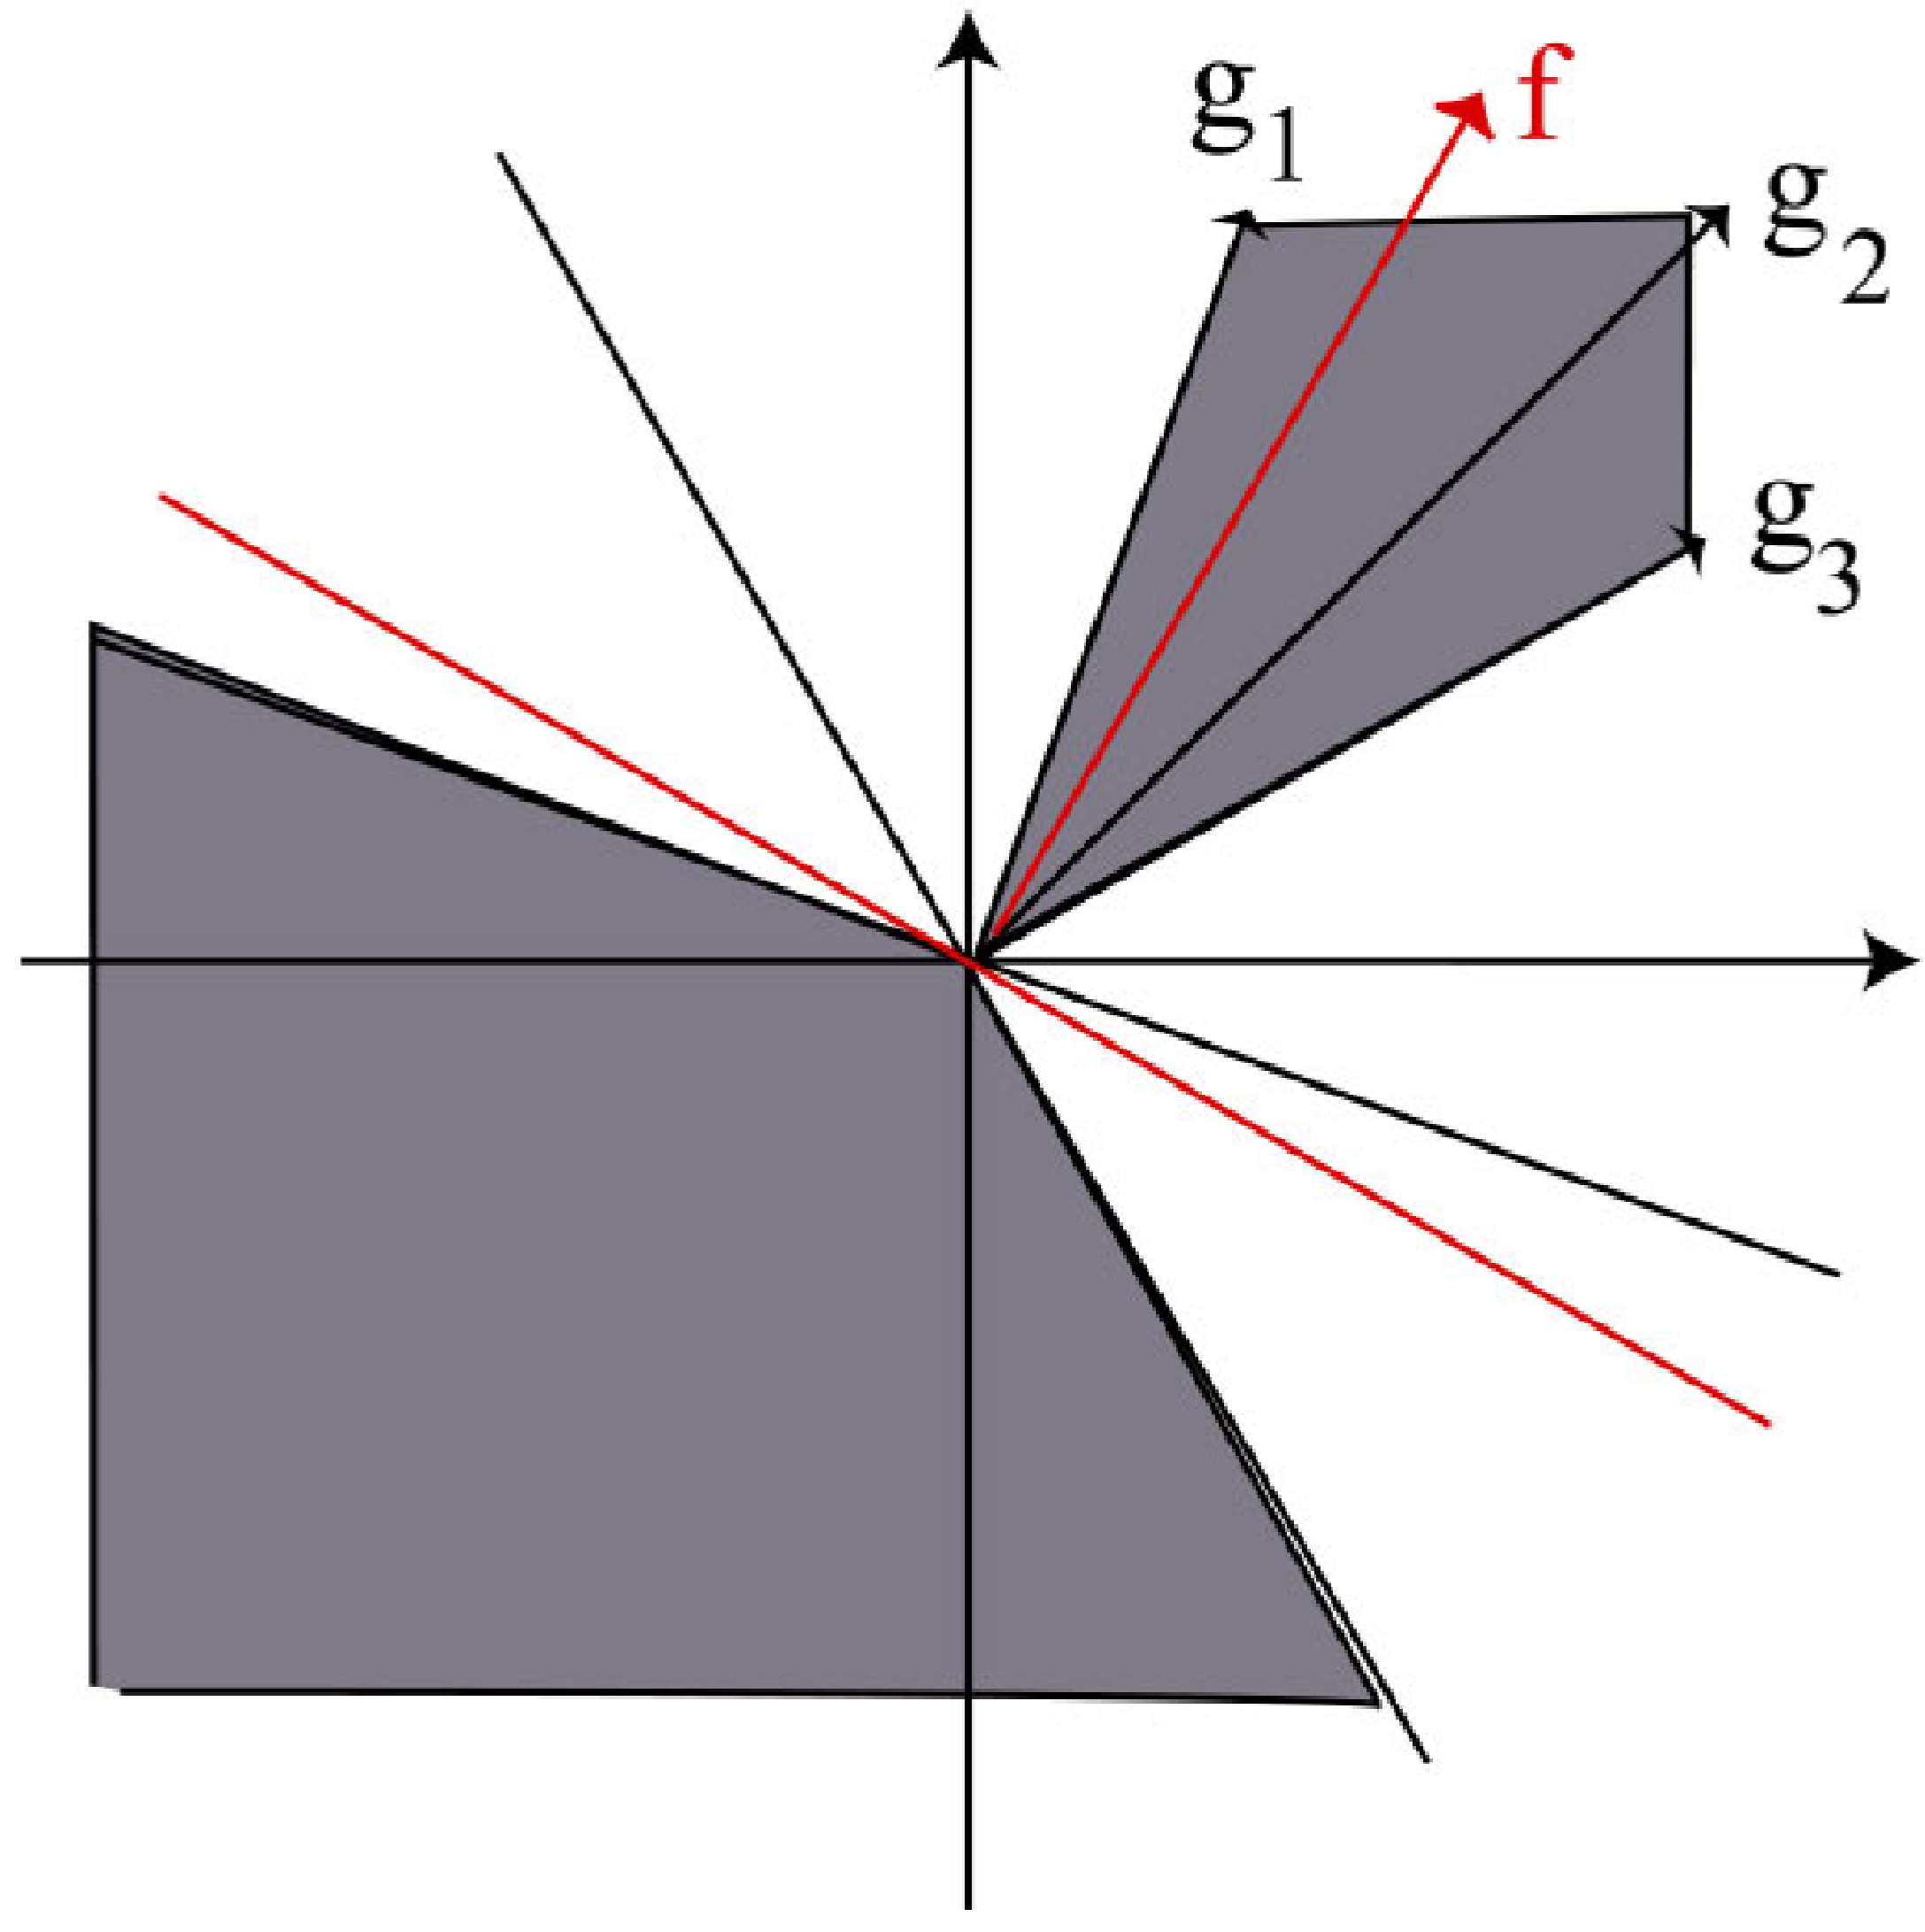
\includegraphics[width=0.45\columnwidth]{img/bdm/mathprog/farkasex}
\end{center}

\subsubsection{Farkas' lemma and local optimality}

We want to apply Farkas' lemma to sift candidate points. Let us map: 
\begin{itemize}
	\item The vectors $g_j$ onto the gradients of the active constraints $\nabla g_j (\tilde x)$
	$$ g_j = \nabla g_j (\tilde x) $$
	
	\item Vector $f$ onto the \textit{antigradient} (opposite of the gradient) of the objective function $- \nabla f (\tilde x)$
	$$ f = - \nabla f (\tilde x) $$
\end{itemize}

The statement of Farkas' lemma becomes
$$ \exists \mu_j \geq 0 : \nabla f (\tilde x) + \sum_{j \in J_a (\tilde x)} \mu_j \nabla g_j (\tilde x) = 0 $$
if and only if
$$ (\nabla f (\tilde x))^T p \geq 0, \quad \forall p : (\nabla g_j (\tilde x))^T p \leq 0, \quad \forall j \in J_a (\tilde x) $$

A vector $p$ with $p^T \nabla g_j (x) \leq 0$, $\forall j \in J_a (x)$ is tangent to a feasible arc. We remove point $x$ when $\nabla f(x)^T p < 0$ for all such vectors. Therefore, \textbf{$x$ is candidate when} $\nabla f(x)^T p \geq 0$ for all feasible tangents, i.e., the second expression in Farkas' lemma, as stated above.

Replacing it with the equivalent first expression, we can tell when a regular point is candidate for local optimality (the first expression is the condition). Don't loop an all $x$ and $p$: solve a system of equations in $\mu$ and $x$.

\subsection{Second geometric interpretation}

The antigradient $- \nabla f(x)$ is the direction of quickest improvement. The gradients of the active constraint $\nabla g_j (x)$ are the directions of quickest violation.

Multipliers $\mu_j \geq 0$ let combination $\sum_{j \in J_a (x)} \mu_j g_j (x)$ describe a cone, denoted as $C_g$, the cone of the gradients of the active constraints.

In candidate points, the antigradient of the objective falls in $C_g$
$$ - \nabla f(x) = \sum_{j \in J_a (x)} \mu_j \nabla g_j (x) $$

When $-\nabla f(x) \in C_g (x)$ the objective improves only violating constraints (\textit{no vector is tangent  to a feasible and improving arc}).

\subsection{Standard form of Karush-Kuhn-Tucker conditions}

In general, KKT-conditions are reported in an equivalent standard form, that has two small modifications. 

The first problem of the analytic conditions is that
$$ \nabla f(x) + \sum_{j \in J_a (x)} \mu_j \nabla g_j (x) = 0 $$
The sum applies only to the constraints active in an unknown point $x$. \textit{How to find them?}

The conditions are reformulated
\begin{enumerate}
	\item Adding the gradients of the nonactive constraints
	$$ \nabla f(x) + \sum_{j = 1}^m \mu_j \nabla g_j (x) = 0 $$
	
	\item Forcing to zero the multipliers of the nonactive constraints 
	$$ \mu_j g_j (x) = 0, \ \text{ for } j = 1, \dots, m $$
\end{enumerate}
These equalities are called the \textbf{complementarity conditions}, as they are equivalent to $g_j (x) < 0 \implies \mu_j = 0$.

Second, we have already seen how equality constraints can be replaced by pairs of inequalities (see \ref{subsub:equalityconstraintsreplaced})., but it's simpler to
\begin{enumerate}
	\item Use a single multiplier $\lambda_i$
	
	\item Relax the nonnegativity condition on the multiplier: $\lambda_i \in \R$
\end{enumerate}

Two opposite gradients with multipliers $\geq 0$ can always be replaced by a single gradient with a multiplier equal to the difference of the original two. In fact
$$ \begin{cases}
	\nabla g_{j_i'} (x) & = \nabla h_i (x) \\
	\nabla g_{j_i''} (x) & = - \nabla h_i (x)
\end{cases}$$
and 
$$ \mu_{j_i'} \nabla g_{j_i'} (x) + \mu_{j_i''} \nabla g_{j_i''} (x) = \left(\mu_{j_i'} - \mu_{j_i''}\right) \nabla h_i (x) = \lambda_i \nabla h_i (x) $$
with $\mu_{j_i'} \geq 0$, $\mu_{j_i''} \geq 0$ and $\mu_{j_i'} - \mu_{j_i''} = \lambda_i$ free in $\R$. \\

\begin{theo}[KKT-conditions]
	Let $X = \left\{x \in \R^n \mid h_i (x) = 0, g_j (x) \leq 0\right\}$, with $i = 1, \dots, s$ and $j = 1, \dots, m$ and $f, h_i, g_j \in C^1 (X)$ for $i = 1, \dots, s$ and $j = 1, \dots, m$. If $x^\ast$ is a regular point in $X$ and a local optimum point for $f$ in $X$, then there exists free multipliers $\lambda_i$ and nonnegative multipliers $\mu_j$ such that:
	$$
	\renewcommand{\arraystretch}{1.35}
	\begin{array}{r l}
		\nabla f \left(x^\ast\right) + \sum_{i = 1}^s \lambda_i \nabla h_i \left(x^\ast \right) + \sum_{j = 1}^m \mu_j \nabla g_j (x^\ast) = 0 & \\
		\mu_j g_j \left(x^\ast \right) = 0 & j = 1, \dots, m \\
		h_i \left(x^\ast \right) = 0 & i = 1, \dots, s \\
		g_j \left(x^\ast\right) \leq 0 & j = 1, \dots, m \\
		\mu_j \geq 0 & j = 1, \dots, m
	\end{array}
	$$
\end{theo}

The "sifting", therefore, does not consist in scanning all points and directions, but it consists of solving a system of equalities and inequalities, identifying all points that satisfy it.

The system consists of $n + s + m$ equations: 
\begin{itemize}
	\item $n$ equations from Farkas' lemma
	
	\item $s$ equations from equality constraints 
	
	\item $m$ equations from the complementarity conditions
\end{itemize}
imposed on $n + s + m$ variables:
\begin{itemize}
	\item $n$ variables to determine the solution $x$ 
	
	\item $s$ variables to determine the multiplier vector $\lambda$
	
	\item $m$ variables to determine the multiplier vector $\mu$
\end{itemize}
and is therefore balanced.

The $2m$ inequalities
\begin{itemize}
	\item $m$ constraints on the solution
	
	\item $m$ nonnegativity conditions on the multipliers
\end{itemize}
remove solutions, but do not decrease freedom degrees (\textit{the number of solutions is probably finite}).

%\subsubsection{Relevant particular cases}
%
%\paragraph{Unconstrained problems} Solved by the classical condition on first derivatives
%$$ \nabla f(x) = 0 \Leftrightarrow \frac{\partial f}{\partial x_i} = 0, \quad \forall i = 1, \dots, n $$
%
%\paragraph{Linear programming} Solved imposing:
%\begin{itemize}
%	\item Farkas' lemma, that corresponds to dual constraints
%	
%	\item The complementarity conditions, that correspond to complementary slackness
%	
%	\item The feasibility constraints, that correspond to the primal constraints
%	
%	\item The nonnegativity conditions, that correspond to the nonnegativity of the dual variables
%\end{itemize}
%
%\paragraph{Discrete problems} On such problems, the conditions are correct, but useless: the integrality constraint
%$$ X \subseteq \Z^n \Leftrightarrow h_i (x) = \sin (\pi x_i) = 0$$
%occurs explicitly in the system and every feasible point is candidate: the KKT condition reduce to the exhaustive algorithm. This is obvious considering that isolated points are locally optimal.
%
%More on the lecture notes.

% End L8